\section{Monte Carlo}

Monte-Carlo methods are a set of randomized algorithms. The general idea is to use random samplings rather than computing to help solve a problem. Such algorithms are mostly used when computing a solution to the problem is not feasible. Because of the use of random samplings, these are heuristic by nature: their results are not always guaranteed to be exact. Throughout the years, Monte-Carlo methods have been successfully used in physics, mathematics  and computer sciences.\\


In this report, we will interest ourselves in a special case of Monte-Carlo methods: Monte-Carlo tree search (MCTS). It applies Monte-Carlo principles to tree exploration. The main field of application is artificial intelligence, especially games with very large move space where a complete tree exploration is not possible in reasonable time, such as Chess and Go.\\

MCTS is composed of four steps : selection, expansion, simulation and backpropagation. These steps are repeated until time runs out, the maximum number of simulated games has been played, a satisfying result is found or whatever condition is relevant. Generally, the more iterations are run, the more accurate is the result.

The selection step chooses a node in order to play a simulation from it. Several algorithms exist for this stage, depending on the context. The expansion step produces children of the selected node if not already generated. This step makes the search tree grow in height. The simulation step plays the game until the end by following nodes selected with a selection algorithm, which can be the same as the one used in the selection step or a different one. Finally, the backpropagation step uses the outcome of the simulated game to modify the estimated value of the nodes traversed. This is the crucial step to know what has been played and whether the selected moves constitute good choices or not.

After playing enough simulated games, a player can then choose amongst the playable moves which one to play using the estimated value of the move. The selection algorithm can be one of the following (from \cite{ChaPHD}) :
\begin{itemize}
\item Max Child : Choosing the node with the highest value.
\item Robust Child : Choosing the node with the highest number of games played.
\item Robust-Max Child : Choosing the node with both the best value and the highest number of games played.
\item Secure Child : Choosing the node maximizing a lower confidence bound.\\
\end{itemize}


\begin{figure}
\centering
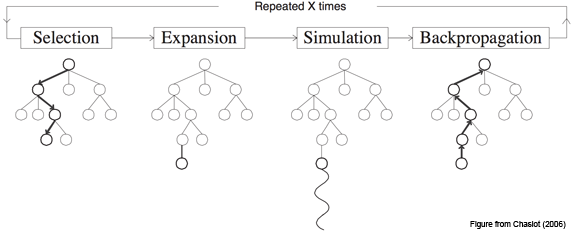
\includegraphics[width=11cm]{mcts-algorithm.png}
\caption{Steps of the Monte-Carlo tree search}
\label{treesearch}
\end{figure}

According to \emph{Guillaume Chaslot} \cite{ChaPHD} : "MCTS is
applicable if at least the following three conditions are satisfied: (1) the payoffs are bounded
(the game scores are bounded), (2) the rules are known (complete information), and (3) simulations terminate relatively fast (game length is limited)". Those three criteria are verified in the case of the map-coloring game. We will use Monte-Carlo tree search to implement an AI capable of playing Alice or Bob.\\

\section{How our AI works}

To modelise a map-coloring game, each node of the exploration tree will contain:
\begin{itemize}
\item The move played when choosing that node, which is simply the node chosen in the game graph and the color used.
\item The total number of games played through that node.
\item The number of games with a favorable outcome for Alice while playing through that node.
\end{itemize}
For each node in the search tree, its value can be seen as the victory ratio for Alice : $\frac{games \ won}{games \ played}$.\\

The selection algorithm we used is based on multi-armed bandit algorithms as described in \cite{MAB}. Indeed, selecting a node amongst the children of the current node in the tree can be seen as a multi-armed bandit problem, where each node is a bandit, its profit being its value. We chose the UCT algorithm, based on the UCB1 multi-armed bandit algorithm, described in \cite{ChaPHD}. This algorithm is called best-first because it always selects the node which seems to be the best. This estimation is based on the value of the node and an upper confidence bound defined as : 
$ \sqrt{\frac{2\ln{n}}{n_j}}$, $n$ being the total number of games played on the parent and $n_j$ being the number of games played on this node.\\

 For every game played through a node, $n$ and $n_j$ grow, thus the upper confidence bound of this node is reduced. This is a formal way of describing an intuitive idea : "The more I play this move, the more I am confident in the value I have calculated". The best node according to the algorithm is the node whose value plus its upper confidence bound is the highest. By using this algorithm, we can quickly stop exploring the least interesting nodes to concentrate on better ones, thus maximizing the profit from a fixed number of simulations.\\

%Introduction du terme zero-sum : pas expliqué, explication nécessaire donc (footnote par exemple ?)
Nevertheless, this algorithm suits well a general Monte-Carlo tree search. In our particular case, we deal with a game between two opponents whose objectives are opposite. Using this algorithm directly would bring us to consider that the opponent is playing toward the same goal, thus helping us, which is of course false. The canonic way of dealing with that problem in a two-player zero-sum\footnote{A game is said to be zero-sum if the winner wins as much as the loser is losing.} game is called Minimax (established in \cite{Minimax}). When exploring a tree with Minimax, the values are maximized when playing with player 1 and minimized when playing player 2, to represent the opposite goal. We reproduced a similar process in the UCT algorithm. If Alice is playing, the confidence interval of the node is added to its value, and the chosen node is the one with the highest resulting total. On the contrary, if Bob is playing, the confidence interval is substracted from the value, resulting in a lower confidence bound. The selected node is then the one with the lowest lower confidence bound.
Using this minimax UCT algorithm, our AI implementation will be the same both for Alice and Bob.\\

The other steps of the Monte-Carlo tree search are now straightforward. The expansion step just generates every legal move on the graph from the current position with the currently used colors, and moves with a new color and adds a node for each one. The simulation step reuses the selection algorithm to play until the game is finished. Finally, the backpropagating step increments the number of games played and won according to the outcome of the game.\\

%Dans Monte Carlo, on va chercher à jouer beaucoup de parties pour un graph donné (que nous appellerons le graph étudié) afin de pouvoir jouer les meilleurs coups possibles. 
%Pour chaque graph étudié, nous générons un arbre des coups joués où chaque nœuds, sauf la racine, correspondent à des coups joués sur ce graph. 
%
%Ce que contient un nœud de l’arbre généré : 
%\begin{itemize}
%\item le nœud joué dans le graph étudié
%\item la couleur jouée sur ce nœud 
%\item le nombre de partie jouées en passant par ce nœud 
%\item le nombre de partie gagné par Alice en passant par ce nœud
%\end{itemize}
%
%Au début l’arbre ne contient que la racine et les premiers coups possibles. Nous n’avons aucune connaissance des coups qui amènent à colorier proprement le graph étudié ni de ceux qui nous mettrons  dans une situation bloquante. 
%
%Afin de limiter le nombre de fils, nous allons éliminé des coups équivalents : nous considérons que les couleurs sont numérotées et qu’il est impossible de jouer une couleur n, si la couleur n-1 n’a pas encore été jouée. En effet il est équivalent d’introduire la couleur n-1 ou la couleur n. 
%
%D’autre part nous allons généré le graph au fur et a mesure des parties et des coups joués. À chaque fois que l’on est dans un nœud (i.e. on viens de jouer le coup correspondant dans le graph étudié), si il n’a pas de fils, on regarde l'état de la partie : 
%\begin{itemize}
%\item soit la partie est finie (Alice a gagné ou Bob à gagné), on remonte alors jusqu’à la racine en mettant à jour tous les nœuds sur le chemin. Si Alice a gagné (i.e. le graph étudié est entièrement colorié) on incrémente le nombre de partie joué et le nombre de partie gagné. Si Alice n’a pas gagné (i.e. le graph étudié n’est pas entièrement colorié)  on incrémente juste le nombre de partie joué.
%\item soit on peut continuer (auquel cas on génère les fils et on continue la simulation récursivement).
%\end{itemize}
%Quand on a joué dans un nœud, on a un pourcentage de victoire pour le coup correspondant, mais il n’est pas forcément représentatif. Le fait de jouer plus de parties va permettre de diminuer l'intervalle de confiance de ce ratio de victoire.
%
%%\subsection {Algorithme de notre IA}
%Pour éviter de toujours passer par les mêmes nœuds, nous allons essayé passer par tous les frères d’un nœud déjà visité avant de pouvoir le revisiter pour explorer ces fils. Ce qui compte, ce sont surtout les coups au premier niveau (le niveau que l’on est en train d’étudier, les coups à jouer immédiatement). Les coups de niveau inférieur ne pourront pas être tous explorés, mais seront regardés de plus près quand on avancera dans le jeu et qu'ils arriveront au premier niveau.
%La partie délicate de Monte-Carlo est la sélection de nœud pour l'exploration. Dans un premier temps nous avons considéré  qu’il faut en priorité visiter le nœud qui a le moins de parties jouées, car il a été visité moins de fois que ses « frères ». Mais jouer celui le moins regardé pour l'instant n'est clairement pas la bonne solution sur le long terme. Il faut une solution adaptative, qui va jouer les coups moins regardés au début, puis qui va jouer les meilleurs pour vérifier que ce sont bien les meilleurs. Nous allons donc utiliser les algorithmes de Multi-armed bandit, plus particulièrement UCB1, qui donne de bons résultats.
%(ressource en anglais : \url{http://www.chrisstucchio.com/blog/2012/bandit_algorithms_vs_ab.html})
%(ressources en français : \url{http://researchers.lille.inria.fr/~munos/master-mva/lecture03.pdf}, \url{http://fr.slideshare.net/cornec/bandits-algo-klucb-par-garivier} )
%La seconde partie de Monte Carlo est l'exploitation. Une fois qu'on a effectué assez de simulations, on choisit un nœud pour le jouer "pour de vrai". Là encore, il y a plusieurs solution : on peut en effet prendre le nœud avec le meilleur ratio brut, mais on peut aussi prendre le nœud avec le meilleur ratio au mieux (plus l'intervalle de confiance) ou encore celui avec le meilleur ratio au pire (moins l'intervalle de confiance). 
%Sinon, pour la différence entre Alice et Bob, on se base sur une sélection min-max classique. Donc pour Alice on choisit le coup qui a le plus grand nombre de partie gagnée. Et pour Bob on choisit celui qui a le plus petit nombre de partie gagnée. 
